\documentclass[12pt]{article}
\usepackage{amsmath}
\usepackage{graphicx}
\usepackage[justification=RaggedRight]{caption}
\usepackage{geometry}
\geometry{a4paper, top=30mm, left=30mm, right=30mm, bottom=30mm}
\usepackage[T1]{fontenc}
\usepackage[utf8]{inputenc}
\usepackage{here}
\setlength{\parindent}{0pt}
\begin{document}
\begin{titlepage}
\centering
\title{\textbf{Viskoelastizität}}
\author{Garnik Arutyunyan \and Marcel Gerhard \and Heinz-Ullrich Rings}
\date{\parbox{\linewidth}{\centering%
		\endgraf\bigskip
		Modellierungspraktikum}}
\maketitle
\thispagestyle{empty}
\end{titlepage}
\newpage

\section{Einführung}

\subsection{Rheologie}
In dieser Modellierung geht es um den Bereich der Lithosphäre. Diese umfasst die Erdkruste und den äußersten Teil des Erdmantels. Das Gestein in dieser Schicht ist fest, zeigt jedoch aufgrund des hohen Drucks und der hohen Temperatur auch viskoses Verhalten. Dies macht eine viskoelastische Betrachtung notwendig.


\subsection{Viskoelastizität}
Ein viskoelastischer Körper weist gleichzeitig viskoses und elastisches Verhalten auf. Als viskoelastischen Modell wird die Maxwell-Rheologie verwendet. Dies lässt sich veranschaulichen durch die Reihenschaltung einer Feder, welche das elastische Verhalten beschreibt, und einem Dämpfungselement, welches das viskose Verhalten beschreibt. Die Verformung ist aufgrund des Dämpfungselementes irreversibel. Dieses rein viskose Verhalten wird um eine elastische Komponente erweitert, welche nur bei Belastung in Erscheinung tritt. Wird das Material deformiert und diese Deformation dann beibehalten, so verschwindet die Spannung mit der Zeit, aufgrund des viskosen Anteils. Man kann also zwischen drei Zeitintervallen unterscheiden:
\begin{itemize}
	\item Instantane elastische Antwort
	\item Relaxation der Scherkräfte auf der Zeitskala der Maxwell-Zeit $t_{Maxwell} = \frac{\mu}{G}$
	\item Lineares Kriechen einer newtonschen Flüssigkeit
\end{itemize}

\subsection{Mathematische Beschreibung}
Mathematisch lässt sich das viskoelastische Verhalten durch die Stokes Gleichungen für inkompressiblen Fluss beschreiben. Der gewählt Ansatz lässt sich wie folgt formulieren:
\begin{equation}
	\epsilon (\nu) = \underbrace{\frac{1}{2\mu}\tau}_{viskos} + \underbrace{\frac{1}{2G}\frac{D\tau}{Dt}}_{elastisch}
	\label{epsilon}
\end{equation}
Die Gleichung (\ref{epsilon}) zeigt, dass die Deformation von Maxwell-viskoelastischen Materialien von der relativen Zusammensetzung von viskosem und elastischem Teil abhängt.
\\
Eine Anforderung an diese Rheologie ist die Berechnung einer genauen Lösung für das Spannungsfeld aufgrund des "Gedächtnisses" der Elastizität.
Man erhält folgende FEM Formulierung für die Maxwell-viskoelastische Rheologie:
		\begin{align*}
&\int_{\Omega} \boldsymbol{B^T} \frac{2\mu \Delta t}{\Delta t + De\mu} \boldsymbol{D'} \boldsymbol{B} \bar{v}^{(k+1)} d\Omega -  \int_{\Omega} \boldsymbol{B^T_{vol}} \boldsymbol{H} \bar{p}^{(k+1)} d\Omega \\ 
&-f  = -\int_{\Omega} \boldsymbol{B^T} \frac{De\mu}{\Delta t + De\mu}(\boldsymbol{I}+\boldsymbol{W})\tau^{*n} d\Omega
\end{align*}
\begin{align*}
\int_{\Omega} \boldsymbol{H^T} \boldsymbol{B_{vol}}  \bar{v}^{(k+1)} d\Omega = g
\end{align*}
Hierbei sind $\boldsymbol{H}, \boldsymbol{B_{vol}}$ Ableitungen der Shapefunktionen und $\boldsymbol{N}, \boldsymbol{H}$ Shapefunktionen. Mit $De$ bezeichnet man die Deborah-Zahl, welche die Zeitabhängigkeit des viskoelastischen Verhaltens wiedergibt. Die Matrizen $\boldsymbol{D'}$ und $\boldsymbol{W}$ bezeichnet man als Rheologiematrix und Jaumann Stress-Rotations-Matrix. In $f$ und $g$ stecken externe Kräfte, sowie Randbedingungen.
\\
In Matrixform lässt sich das Problem wie folgt formulieren: \\
\newline
\begin{center}
	$\begin{bmatrix}
	K_{vv} & K_{vp} \\
	K_{pv} & 0 \\
	\end{bmatrix}
	\begin{Bmatrix}
	\bar{v}^{(k+1)} \\
	\bar{p}^{(k+1)}
	\end{Bmatrix}
	= \begin{Bmatrix}
	f \\
	g
	\end{Bmatrix}$
\end{center}



\section{Code}
Unser Code basiert auf dem Stokes Löser von Aufgabenblatt 3. Hierbei nutzen wir nur den Faktor $mu=\frac{1}{\frac{1}{\mu}+\frac{1}{G\Delta t}}$ anstelle von $\mu$ bei der Erstellung der Matrix Kvv. Außerdem wird dem Lastvektor der elastische Teil
\begin{equation*}
	\int_{\Omega}^{} \boldsymbol{B^T} \frac{1}{1+\frac{G\Delta t}{\mu}}(\boldsymbol{I}+\boldsymbol{W})\tau d\Omega
\end{equation*}
hinzugefügt. Hierbei wird $\tau$ in jedem Integrationspunkt durch
\begin{equation*}
	\tau = \frac{E}{(1-\nu)^2} \begin{bmatrix}
	1 & \nu & 0 \\
	\nu & 1 & 0 \\
	0 & 0 & \frac{1-\nu}{2} \\
	\end{bmatrix}
	\boldsymbol{B}\Delta u
\end{equation*}
berechnet, wobei $\Delta u$ die Verschiebung in den Integrationspunkten des Rechtecks ist. \\
Um eine einfachere Umsetzung des Schiebens von beiden Seiten zu ermöglichen, haben wir uns entschlossen, mit einer festen Geschwindigkeit von beiden Seiten zu drücken. \\
Da wir nach jedem Zeitschritt unser Gitter verschieben, muss unsere FEM im Gegensatz zu der Aufgabe auch mit beliebigen Vierecken arbeiten.

\section{Ergebnisse}
Im folgenden werden die Ergebnisse unserer Implementierung dargestellt. \\
\newline
Im ersten Teil betrachten wir ein Gebiet mit $(0,1)^2$. Für eine über das gesamte Gebiet homogene Viskosität erhält man folgende Ergebnisse: \\

\begin{figure}[H]
	\begin{minipage}[hbt]{0.25\textwidth}
		\centering
		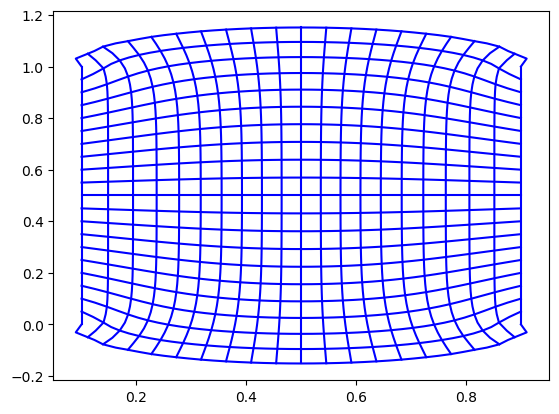
\includegraphics[width=5cm]{A1_Gitterverschiebung.png}
		\caption{Gitterverschiebung nach 10 Jahren}
		\label{Bild1}
	\end{minipage}
	\hfill
	\begin{minipage}[hbt]{0.25\textwidth}
		\centering
		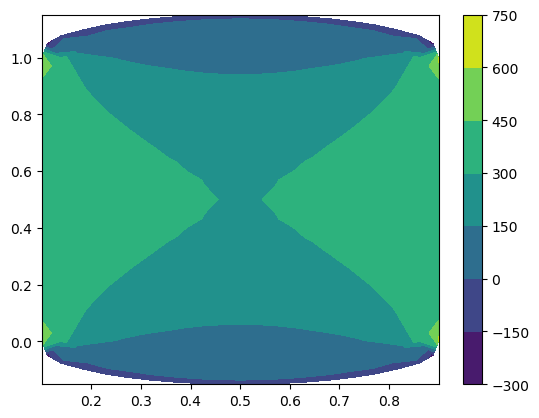
\includegraphics[width=5cm]{A1_Druck.png}
		\caption{Druckverteilung nach 10 Jahren}
		\label{Bild2}
	\end{minipage}
\hfill
	\begin{minipage}[hbt]{0.25\textwidth}
	\centering
	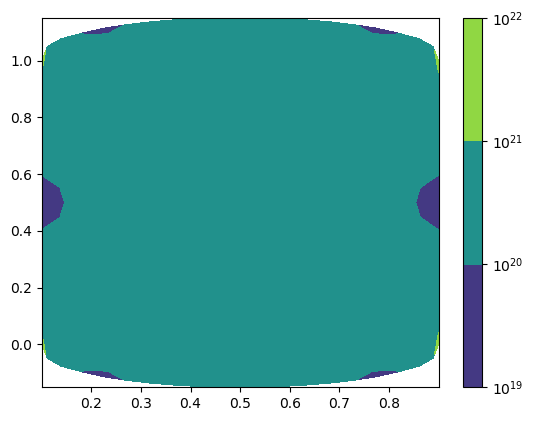
\includegraphics[width=5cm]{A1_tau2nd.png}
	\caption{$\tau$ nach 10 Jahren}
	\label{Bild2}
\end{minipage}
\end{figure}
.


\begin{figure}[H]
	\begin{minipage}[hbt]{0.25\textwidth}
		\centering
		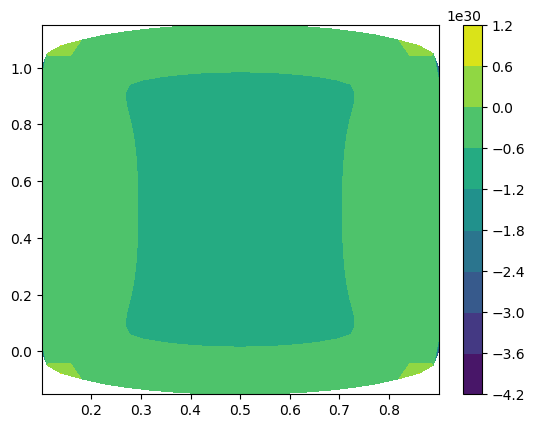
\includegraphics[width=5cm]{A1_tauxx.png}
		\caption{$\tau_{xx}$ nach 10 Jahren}
		\label{Bild1}
	\end{minipage}
	\hfill
	\begin{minipage}[hbt]{0.25\textwidth}
		\centering
		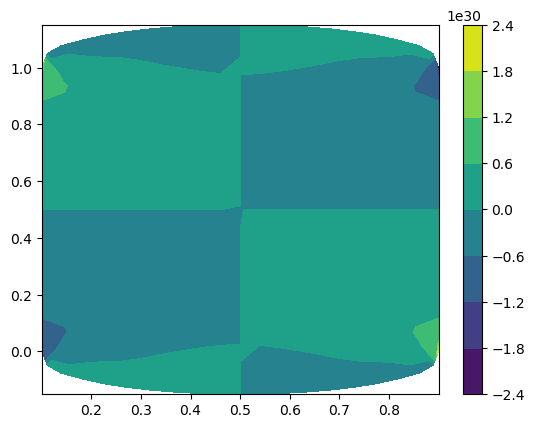
\includegraphics[width=5cm]{A1_tauyy.png}
		\caption{$\tau_{yy}$ nach 10 Jahren}
		\label{Bild2}
	\end{minipage}
	\hfill
	\begin{minipage}[hbt]{0.25\textwidth}
		\centering
		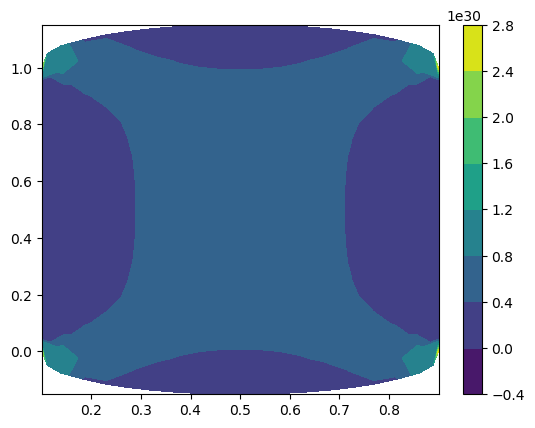
\includegraphics[width=5cm]{A1_tauxy.png}
		\caption{$\tau_{xy}$ nach 10 Jahren}
		\label{Bild2}
	\end{minipage}
\end{figure}


Die folgenden Ergebnisse zeigen das Verhalten des Materials bei gleichgroßen Schichten unterschiedlicher Viskositäten. In aufsteigender Folge ist die Viskosität $10^{23}$, $10^{20}$, $10^{15}$, $10^{17}$, $10^{20}$.
\begin{figure}[H]
	\begin{minipage}[hbt]{0.25\textwidth}
		\centering
		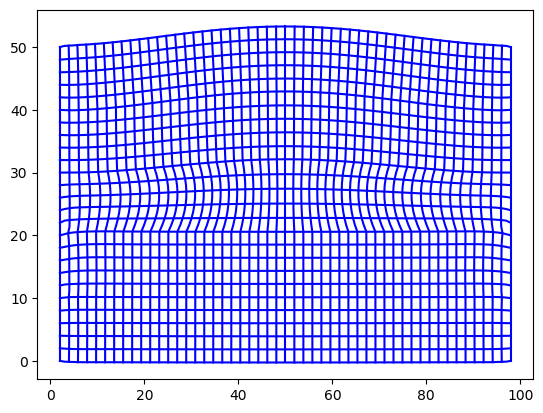
\includegraphics[width=5cm]{A2_Gitterverschiebung_2000.png}
		\caption{Gitterverschiebung nach 2000 Jahren}
		\label{Bild1}
	\end{minipage}
	\hfill
	\begin{minipage}[hbt]{0.25\textwidth}
		\centering
		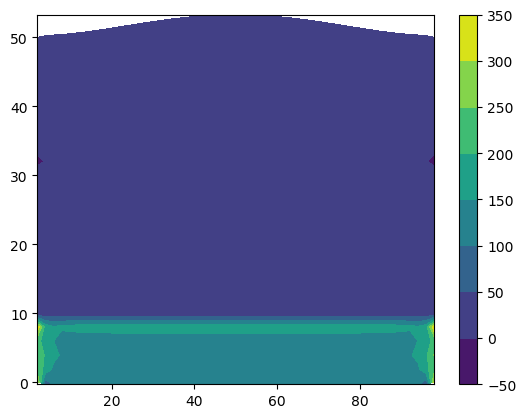
\includegraphics[width=5cm]{A2_Druck_2000.png}
		\caption{Druckverteilung nach 2000 Jahren}
		\label{Bild2}
	\end{minipage}
	\hfill
	\begin{minipage}[hbt]{0.25\textwidth}
		\centering
		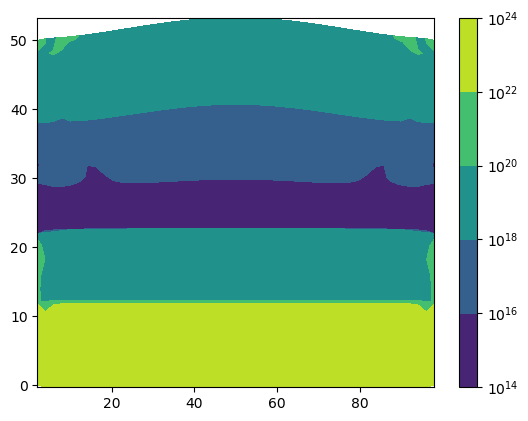
\includegraphics[width=5cm]{A2_tau2nd_2000.png}
		\caption{$\tau$ nach 2000 Jahren}
		\label{Bild2}
	\end{minipage}
\end{figure}
.


\begin{figure}[H]
	\begin{minipage}[hbt]{0.25\textwidth}
		\centering
		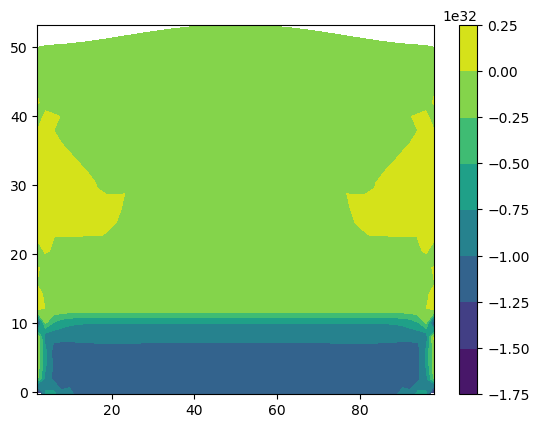
\includegraphics[width=5cm]{A2_tauxx_2000.png}
		\caption{$\tau_{xx}$ nach 2000 Jahren}
		\label{Bild1}
	\end{minipage}
	\hfill
	\begin{minipage}[hbt]{0.25\textwidth}
		\centering
		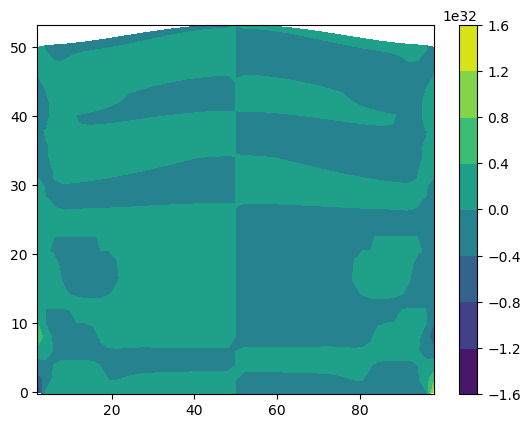
\includegraphics[width=5cm]{A2_tauyy_2000.png}
		\caption{$\tau_{yy}$ nach 2000 Jahren}
		\label{Bild2}
	\end{minipage}
	\hfill
	\begin{minipage}[hbt]{0.25\textwidth}
		\centering
		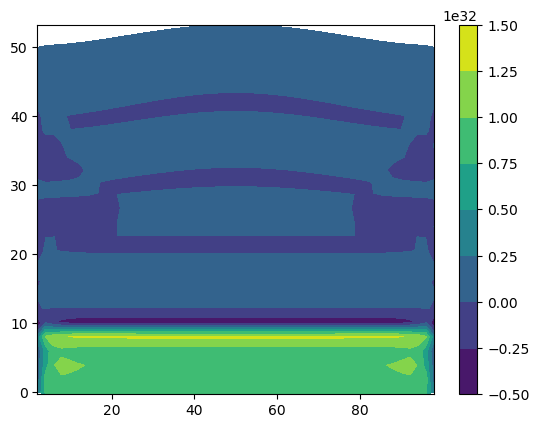
\includegraphics[width=5cm]{A2_tauxy_2000.png}
		\caption{$\tau_{xy}$ nach 2000 Jahren}
		\label{Bild2}
	\end{minipage}
\end{figure}

Nach der doppelten Zeit erhält man folgendes:

\begin{figure}[H]
	\begin{minipage}[hbt]{0.25\textwidth}
		\centering
		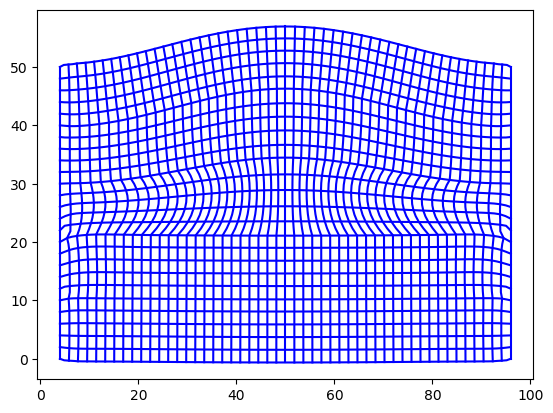
\includegraphics[width=5cm]{A2_Gitterverschiebung_4000.png}
		\caption{Gitterverschiebung nach 4000 Jahren}
		\label{Bild1}
	\end{minipage}
	\hfill
	\begin{minipage}[hbt]{0.25\textwidth}
		\centering
		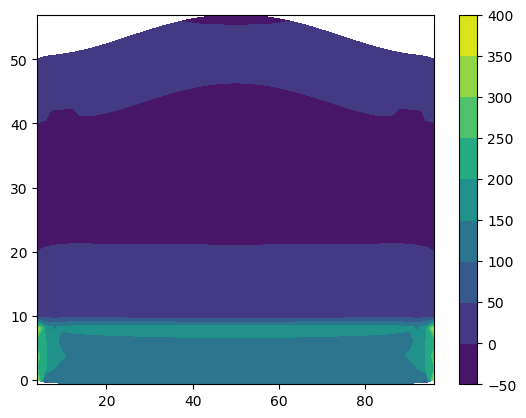
\includegraphics[width=5cm]{A2_Druck_4000.png}
		\caption{Druckverteilung nach 4000 Jahren}
		\label{Bild2}
	\end{minipage}
	\hfill
	\begin{minipage}[hbt]{0.25\textwidth}
		\centering
		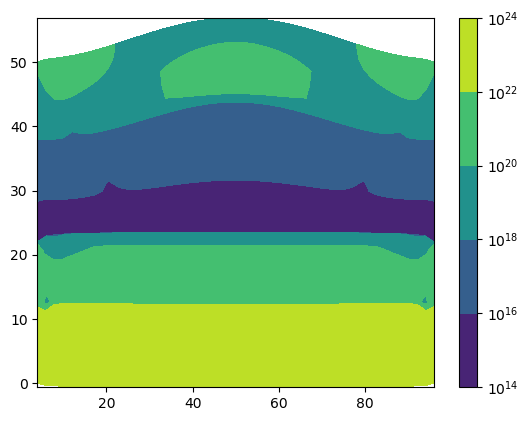
\includegraphics[width=5cm]{A2_tau2nd_4000.png}
		\caption{$\tau$ nach 4000 Jahren}
		\label{Bild2}
	\end{minipage}
\end{figure}
.


\begin{figure}[H]
	\begin{minipage}[hbt]{0.25\textwidth}
		\centering
		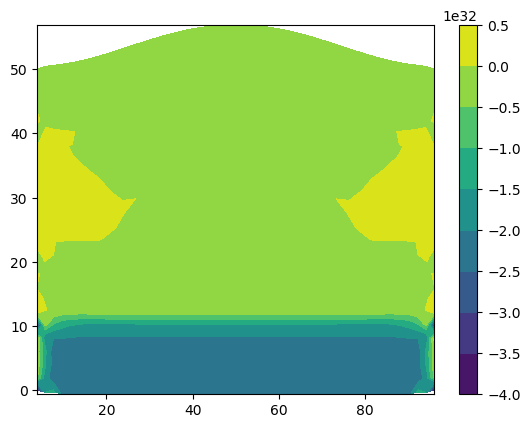
\includegraphics[width=5cm]{A2_tauxx_4000.png}
		\caption{$\tau_{xx}$ nach 4000 Jahren}
		\label{Bild1}
	\end{minipage}
	\hfill
	\begin{minipage}[hbt]{0.25\textwidth}
		\centering
		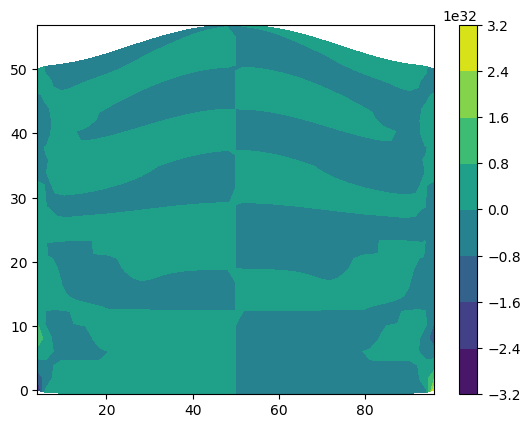
\includegraphics[width=5cm]{A2_tauyy_4000.png}
		\caption{$\tau_{yy}$ nach 4000 Jahren}
		\label{Bild2}
	\end{minipage}
	\hfill
	\begin{minipage}[hbt]{0.25\textwidth}
		\centering
		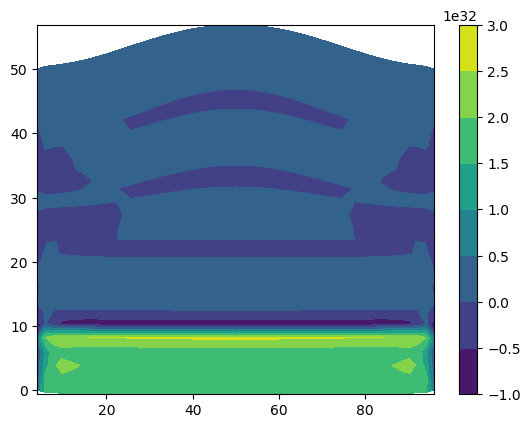
\includegraphics[width=5cm]{A2_tauxy_4000.png}
		\caption{$\tau_{xy}$ nach 4000 Jahren}
		\label{Bild2}
	\end{minipage}
\end{figure}

\end{document}